%%%%%%%%%%%%%%%%%%%%%%%%%%%%%%%%%%%%%%%%%%%%%%%%%%%%%%%%%%%%%%%%%%%%%%%%%%%%%%%
%%%% Problem 1
%%%%%%%%%%%%%%%%%%%%%%%%%%%%%%%%%%%%%%%%%%%%%%%%%%%%%%%%%%%%%%%%%%%%%%%%%%%%%%%
\problem{1}
\subsubsection{Question}
% Keywords
	\index{mechanics!Vehicle's resonant bouncing}

A \SI{1000}{\kg} automobile has ground clearance of \SI{18}{\cm} but when
loaded with an extra \SI{500}{\kg} from its 4 passengers it only clears the
ground by \SI{12}{\cm}. The car's shock absorbers are ineffective. At what
speed (in miles per hour) will the car bounce in resonance when it travels
along a smooth road containing transverse tar patches every \SI{15}{\m}?
Assume that the front and rear suspensions have the same bouncing frequency.

\subsubsection{Answer}

To find the natural resonant frequency of the vehicle, we use the two data
points about it's clearance to obtain the spring constant $k$. We know that
a constant force on a spring system does not change the dynamics, so it's
only the change in mass and distance which are relevant. Therefore by simple
equilibrium requirements,
\begin{align*}
    k ΔL &= mg \\
    k &= \frac{mg}{ΔL}
\end{align*}
where $m$ and $M$ are the masses of the passengers and empty car respectively
and $ΔL$ is the difference in the clearance between the unloaded and loaded
car.

Next, we know that the resonant frequency of a simple harmonic oscillator is
given by $ω = \sqrt{k/m_\mathrm{tot}}$, so
\begin{align*}
    ω &= \sqrt{\frac{mg}{(M+m)ΔL}} \\
    f &= \frac{1}{2π} \sqrt{\frac{mg}{(M+m)ΔL}}
\end{align*}
where the second line has converted from angular to linear frequency. We then
simply relate that to how often the car hits a tar patch and solve for the
velocity. Letting $v$ be the velocity of the car and $d$ be the separation
distance between tar patches,
\begin{align*}
    \frac{v}{d} &= f \\
    v &= \frac{d}{2π} \sqrt{\frac{mg}{(M+m)ΔL}}
\end{align*}
Plugging in the numbers,
\begin{align}
    \boxed{
    v = \SI{17.62}{\m\per\s} = \SI{39.42}{mph}
    }
\end{align}

%%%%%%%%%%%%%%%%%%%%%%%%%%%%%%%%%%%%%%%%%%%%%%%%%%%%%%%%%%%%%%%%%%%%%%%%%%%%%%%
%%%% Problem 3
%%%%%%%%%%%%%%%%%%%%%%%%%%%%%%%%%%%%%%%%%%%%%%%%%%%%%%%%%%%%%%%%%%%%%%%%%%%%%%%
\problem{3}
\subsubsection{Question}
% Keywords
	\index{thermodynamics!Mean free path of helium}
	\index{statistical mechanics!Mean free path of helium}

The cross-section for collisions between helium atoms is about \SI{e-16}{
\cm\squared}. Estimate the mean free path of helium atoms in helium gas at
atmospheric pressure and temperature.

\subsubsection{Answer}

Consider the path traced out by a helium atom as it travels a path length $L$,
colliding with other helium atoms along the way. Given that the cross section
of helium is $σ$, than we can estimate the volume that contains probable
interactions with our atom of interest as $\mathcal V = σL$. To get the number
of interactions, we make use of the fact that we're treating the gas as an
ideal gas. From the ideal gas law,
\begin{align*}
    PV &= NkT
\intertext{so that solving for the number density}
    n = \frac{N}{V} &= \frac{P}{k_B T}
\end{align*}
Combining the density with the volume, we get the number of other [point
particle] helium atoms that are contained within the given helium atom's
interaction volume. If we then assume that the atom interacts with all other
atoms within the volume, and that the collisions are spaced out equally in
time, we just have to normalize the value by the trajectory's path length to
get an estimate of the mean free path of helium in a helium gas:
\begin{align*}
    λ &= \frac{n\mathcal V}{L} = \frac{σP}{k_B T}
\end{align*}
Plugging in $σ = \SI{e-16}{\cm\squared}$, $P = \SI{1.013e5}{\Pa}$, $k_B =
\SI{1.38e-23}{\J\per\K}$, and $T = \SI{298}{\K}$, we get
\begin{align}
    \boxed{
    λ = \SI{4.06}{\micro\m}
    }
\end{align}

%%%%%%%%%%%%%%%%%%%%%%%%%%%%%%%%%%%%%%%%%%%%%%%%%%%%%%%%%%%%%%%%%%%%%%%%%%%%%%%
%%%% Problem 6
%%%%%%%%%%%%%%%%%%%%%%%%%%%%%%%%%%%%%%%%%%%%%%%%%%%%%%%%%%%%%%%%%%%%%%%%%%%%%%%
\problem{6}
\subsubsection{Question}
% Keywords
	\index{mechanics!Tension in a supported rope}

A single closed loop of chain with mass $m$ and length $L$ rests
horizontally on a smooth frictionless con with half-angle $α$. What is the
tension in the chain?

\subsubsection{Answer}

\begin{figure}[H]
    \centering
    \begin{subfigure}[b]{0.49\textwidth}
	\centering
	\begin{tikzpicture}
	    % Draw the triangle
	    \draw (0,0) -- (0,6) -- (4,0) -- cycle;

	    % Add the arc and label to the given angle
	    \draw (0,5.2) arc (-90:-56.31:0.8) coordinate (angle end);
	    \node [anchor=north west] at ($(0,5.2)!0.25!(angle end)$) {$α$};

	    % Pic an arbitrary point along the surface of the cone to represent
	    % the chain length element.
	    \coordinate (point) at ($(0,6)!0.6!(4,0)$);
	    \draw (point) node [fill,black,circle,inner sep=2pt] {};

	    % Draw the gravitational vector from the point
	    \draw [thick,->] (point) -- ++(0,-1)
		node [anchor=north] {$\vec F_g$};

	    % And the normal vector
	    \path [name path=Ny proj] ($(point)+(0,1)$) -- ($(point)+(2,1)$);
	    \path [name path=N vec] (point) -- ($(point)!1!90:(4,0)$);
	    \draw [name intersections={of=Ny proj and N vec, by=x}]
		[thick,->] (point) -- (x)
		node [anchor=south west] {$\vec N$}
		coordinate (norm end);

	    % Draw projections of the normal vector
	    \draw [thick,dashed] (point) -- ++(0,1) -- (norm end);
	\end{tikzpicture}
	\caption{Side View}
    \end{subfigure}
    \hfil
    \begin{subfigure}[b]{0.49\textwidth}
	\centering
	\begin{tikzpicture}
	    % Setup some coordinates:
	    \def\alpha{20}
	    \def\r{5cm}
	    \def\dr{0.2cm}
	    \def\Nr{1cm}
	    
	    \coordinate (center left)  at ($(90+\alpha:\r)$);
	    \coordinate (center mid)   at (90:\r);
	    \coordinate (center right) at ($(90-\alpha:\r)$);

	    \coordinate (outer left)   at ($(90+\alpha:\r+\dr)$);
	    \coordinate (outer mid)    at ($(90:\r+\dr)$);
	    \coordinate (outer right)  at ($(90-\alpha:\r+\dr)$);

	    \coordinate (inner left)   at ($(90+\alpha:\r-\dr)$);
	    \coordinate (inner mid)    at ($(90:\r-\dr)$);
	    \coordinate (inner right)  at ($(90-\alpha:\r-\dr)$);
	    
	    % Draw the radii
	    \draw [dashed] (0,0) -- (center left);
	    \draw [dashed] (0,0) -- (center mid);
	    \draw [dashed] (0,0) -- (center right);
	    % And label them
	    \node [anchor=west] at ($(0,0)!0.5!(center mid)$)   {$r$};
	    \node [anchor=west] at ($(0,0)!0.5!(center right)$) {$r$};

	    % Draw the chain
	    \draw [thick] (inner left) -- (outer left)
		arc (90+\alpha:90-\alpha:\r+\dr) -- (inner right)
		arc (90-\alpha:90+\alpha:\r-\dr);

	    % Draw the normal force
	    \draw (center mid) node [fill,black,circle,inner sep=2pt] {}
		node [anchor=west] {$ds$}
		[very thick,->] -- ++(0,\Nr)
		node [anchor=south] {$\vec N_r$};

	    % Finally, draw the tension vectors
	    \path [name path=Nr] ($(center mid)+(-4,-\Nr)$) -- ++(8,0);
	    \path [name path=Tl]
		(center left) -- ($(center left)!2.5cm!-90:(0,0)$);
	    \path [name path=Tr]
		(center right) -- ($(center right)!2.5cm!90:(0,0)$);

	    \draw [name intersections={of=Nr and Tl, by=x}]
		[very thick,->] (center left) -- (x)
		coordinate (left T end)
		node [anchor=north east] {$\vec T$};
	    \draw [name intersections={of=Nr and Tr, by=x}]
		[very thick,->] (center right) -- (x)
		coordinate (right T end)
		node [anchor=north west] {$\vec T$};
	    \draw [dashed] (left T end) -- (right T end);

	    % Add the known angles
	    \draw ($(0,0)!1cm!(center left)$) arc (90+\alpha:90-\alpha:1cm);
	    \node [anchor=south] at (0,1) {$dφ$};
	    \draw ($(left T end)!1cm!(center left)$) arc (\alpha:0:1cm)
		node [anchor=north] {$\frac 12 dφ$};
	\end{tikzpicture}
	\caption{Top View}
    \end{subfigure}
\end{figure}

Consider just a small element of the chain of arc length $ds$. It will have
a corresponding mass $dm = λ\,ds$ where $λ = m/L$. Knowing that it's a statics
problem, we can easily determine the normal force by balancing the vertical
component with that of gravity.
\begin{align*}
    F_g &= N \sin α \\
    N &= \frac{λg\,ds}{\sin α}
\end{align*}
This leaves the horizontal component of the normal force to be balanced with
the tension within the chain.

Now switching to the top view, we consider the short chain segment $ds$, shown
above with an exagerated curvature. We note that the radial part of the
normal force must be opposed by the sum of the radial components of the two
tensions $T$ acting on the end of the chain segment. By geometry, we know that
the angle with respect to the midpoint's tangent is one half the differential
angle change $dφ = ds/r$. This means we balance the forces as
\begin{align*}
    2T\sin(\frac 12 dφ) &= N \cos α \\
    2T\sin(\frac 12 dφ) &= λg\,ds \cot α
\end{align*}
By the small angle approximation, $\sin (\frac 12 dφ) ≈ \frac 12 dφ$, so after
substituting for the fact that $dr = L/2π$ and $λ = M/L$,
\begin{align}
    \boxed{
    T = \frac{Mg}{2π} \cot α
    }
\end{align}

%%%%%%%%%%%%%%%%%%%%%%%%%%%%%%%%%%%%%%%%%%%%%%%%%%%%%%%%%%%%%%%%%%%%%%%%%%%%%%%
%%%% Problem 8
%%%%%%%%%%%%%%%%%%%%%%%%%%%%%%%%%%%%%%%%%%%%%%%%%%%%%%%%%%%%%%%%%%%%%%%%%%%%%%%
\problem{8}
\subsubsection{Question}
% Keywords
	\index{electrodynamics!LR circuit}

In the figure below, $\mathcal E = \SI{100}{\V}$, $R₁ = \SI{5}{\ohm}$,
$R₂ = \SI{10}{\ohm}$, $R₃ = \SI{15}{\ohm}$, and $L = \SI{1.0}{\henry}$. Find
the values of the currents $I₁$ and $I₂$
\begin{enumerate}[a)]
    \item immediately after the switch $S$ is closed,
    \item a long time later,
    \item immediately after switch $S$ is opened again,
    \item and then how long must you wait, after the switch is opened, before
	$I₂$ falls by a factor of $e$?
\end{enumerate}

\begin{center}
    \vspace{\baselineskip}
    \begin{circuitikz}
	\draw
	    (0,0)
		to[battery,l_=$\mathcal E$]
	    ++(0,3)
		to[closing switch,l_=$S$]
	    ++(3,0)
		to[resistor,l_=$R₁$]
	    ++(3,0)
		coordinate (I2 I3 break)
		to[resistor,l_=$R₃$,i=$I₃$]
	    ++(3,0)
		to[inductor,l_=$L$]
	    ++(0,-3)
		--
	    ++(-3,0)
		coordinate (I2 I3 combine)
		to[short,i=$I₁$]
	    (0,0)
	;
	\draw
	    (I2 I3 break)
		to[resistor,l_=$R₂$,i=$I₂$]
	    (I2 I3 combine)
	;
    \end{circuitikz}
    \vspace{\baselineskip}
\end{center}

\subsubsection{Answer}

Start by applying Kirchoff's rules to the circuit: current is conserved and
the voltage changes must sum to zero around each loop, so
\begin{align}
    I₁ &= I₂ + I₃
	\label{eqn:sp2002p1.8:kirchoff_current} \\
    0 &= \mathcal E - I₁R₁ - I₂R₂
	\label{eqn:sp2002p1.8:kirchoff_leftloop} \\
    0 &= -I₃R₃ - L \frac{dI₃}{dt} + I₂R₂
	\label{eqn:sp2002p1.8:kirchoff_rightloop}
\end{align}

Since only (\ref{eqn:sp2002p1.8:kirchoff_rightloop}) has a term involving
a time derivative, we choose to first solve for the current $I₃$. By solving
for $I₂R₂$ in (\ref{eqn:sp2002p1.8:kirchoff_leftloop}) and substituting,
we eliminate $I₂$ and have
\begin{align}
    0 &= -I₃R₃ - L\frac{dI₃}{dt} + \mathcal E - I₁R₁
    \label{eqn:sp2002p1.8:right_noI2}
\end{align}
Furthermore, by also substituting the value of $I₂$ into
(\ref{eqn:sp2002p1.8:kirchoff_current}):
\begin{align}
    I₁ &= \frac{\mathcal E}{R₁+R₂} + \frac{R₂}{R₁+R₂} I₃
    \label{eqn:sp2002p1.8:current_noI2}
\end{align}
Then by combining (\ref{eqn:sp2002p1.8:right_noI2}) and
(\ref{eqn:sp2002p1.8:current_noI2}), we can produce a differential equation
for $I₃$:
\begin{align*}
    -I₃R₃ - L\frac{dI₃}{dt} + \mathcal E - \frac{R₁}{R₁+R₂}\mathcal E -
	\frac{R₁R₂}{R₁+R₂}I₃ = 0
    \\
    -\underbrace{\frac{R₁R₂ + R₁R₃ + R₂R₃}{R₁+R₂}}_{R'}I₃ = L\frac{dI₃}{dt}
	- \frac{R₂}{R₁+R₂} \mathcal E
\end{align*}
\begin{align}
    \frac{dI₃}{dt} = -\frac{R'}{L} I₃ + \frac{1}{L}\frac{R₂}{R₁+R₂}\mathcal E
	\label{eqn:sp2002p1.8:diffeq_I3}
\end{align}
Considering just the homogenous part, we easily solve it to find the standard
exponential solution
\begin{align*}
    I_{3h}(t) &= I_{30} e^{-R't/L}
\end{align*}
And using the ansatz $I_{3p}(t) = At + B$ for the inhomogenous part,
\begin{align*}
    A &= -\frac{R'}{L}At - \frac{R'}{L}B + \frac 1L\frac{R₂}{R₁+R₂}\mathcal E
    \\
    A &= 0 \\
    B &= \frac{1}{R'}\frac{R₂}{R₁+R₂}\mathcal E
\end{align*}
At $t = 0$, the inductor has no current passing through it, so when the switch
is closed, the current must remain continuous. This gives us the initial
condition necessary to solve for the unknown $I_{30}$, and after doing so
and simplifying, the total solution is
\begin{align}
    I₃(t) &= \frac{\mathcal E}{R'}\frac{R₂}{R₁+R₂}(1 - e^{-R't/L})
	\label{eqn:sp2002p1.8:I3_charging}
\end{align}

Then by substiting this solution back into (\ref{eqn:sp2002p1.8:current_noI2})
we get the solution for $I₁$:
\begin{align}
    I₁(t) &= \frac{\mathcal E}{R₁+R₂} \left[ 1 + \frac{1}{R'}
	\frac{{R₂}²}{R₁+R₂} (1 - e^{-R't/L}) \right]
	\label{eqn:sp2002p1.8:I1_charging}
\end{align}
Finally, combining both inserting both solutions for $I₁$ and $I₃$ into
(\ref{eqn:sp2002p1.8:kirchoff_current}), the solution for $I₂$ is
\begin{align}
    I₂(t) &= \frac{\mathcal E}{R₁+R₂} \left[ 1 - \frac{1}{R'}
	\frac{R₁R₂}{R₁+R₂} (1 - e^{-R't/L}) \right]
	\label{eqn:sp2002p1.8:I2_charging}
\end{align}

Plugging in all of the given values, we find that the currents at the instant
the switch is closed are
\begin{align}
    \boxed{I₁(0) = \SI{6.66}{\A}\quad\quad\text{$S$ is closed}} \\
    \boxed{I₂(0) = \SI{6.66}{\A}\quad\quad\text{$S$ is closed}}
\end{align}
For a long time later, we can let $t \rightarrow ∞$ and find that
\begin{align}
    \boxed{I₁(∞) = \SI{9.09}{\A}\quad\quad\text{$S$ is closed}} \\
    \boxed{I₂(∞) = \SI{5.54}{\A}\quad\quad\text{$S$ is closed}}
\end{align}

Right after the switch is opened, the left loop is taken out of the circuit,
so we immediately know that the value of $I₁$ is zero.
\begin{align}
    \boxed{I₁(0) = 0\quad\quad\text{$S$ is open	}}
\end{align}
For the right loop, we start by noting that the steady state current through
the inductor will be needed. Taking the limit of (\ref
{eqn:sp2002p1.8:I3_charging}), we have that the new initial condition is
\begin{align*}
    I₃(0) &= \frac{\mathcal E}{R'}\frac{R₂}{R₁+R₂}
\end{align*}
$I₂$ now is equal to $-I₃$ since there is no other path for the current to
traverse. This loop's differential equation is then
\begin{align*}
    -(R₂+R₃)I₃ - L\frac{dI₃}{dt} = 0
\end{align*}
Solving for the exponential and using the initial condition above, the time
solution is
\begin{align*}
    I₃(t) &= \frac{\mathcal E}{R'}\frac{R₂}{R₁+R₂} e^{-(R₂+R₃)t/L} \\
    I₂(t) &= -\frac{\mathcal E}{R'}\frac{R₂}{R₁+R₂} e^{-(R₂+R₃)t/L}    
\end{align*}
Therefore the current in $I₂$ just after the switch is opened reverses
direction
\begin{align}
    \boxed{I₂(0) = \SI{-3.64}{\A}}
\end{align}
Then by simple exponential relations, we know that the time time to decay by
a factor of $e$ is given by the reciprocal of the coefficient of $t$, so
inserting the appropriate numbers
\begin{align}
    \boxed{t_\mathrm{decay} = \SI{0.04}{\s}}
\end{align}

%%%%%%%%%%%%%%%%%%%%%%%%%%%%%%%%%%%%%%%%%%%%%%%%%%%%%%%%%%%%%%%%%%%%%%%%%%%%%%%
%%%% Problem 9
%%%%%%%%%%%%%%%%%%%%%%%%%%%%%%%%%%%%%%%%%%%%%%%%%%%%%%%%%%%%%%%%%%%%%%%%%%%%%%%
\problem{9}
\subsubsection{Question}
% Keywords
	\index{thermodynamics!Arbitrary engine efficiency}

An engine using \SI{1}{\mol} of an ideal diatomic gas performs the cycle $A
\rightarrow B \rightarrow C \rightarrow A$ as shown in the diagram below. $A
\rightarrow B$ is an adiabatic expansion, $B \rightarrow C$ occurs at
constant pressure, and $C \rightarrow A$ takes place at constant volume.
What is the efficiency of the cycle?

\begin{center}
    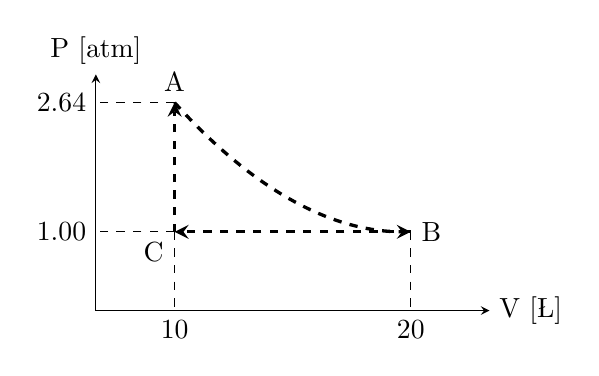
\begin{tikzpicture}[
	>=stealth
    ]
    % Draw the axes
	\draw [->] (0,0) -- (0,3) node [anchor=south] { P [\si{atm}] };
	\draw [->] (0,0) -- (5,0) node [anchor=west] {V [\si{\L}]};

	% Then draw the engine cycle
	\draw [very thick,dashed,->] (1,1)    -- (1, 2.64)
	    node [anchor=south] {A};
	\draw [very thick,dashed,->] (1,2.64) parabola[bend at end] (4,1)
	    node [anchor=west] {B};
	\draw [very thick,dashed,->] (4,1)    -- (1,1)
	    node [anchor=north east] {C};
	;

	% Then draw in the labels that give the absolute numbers
	\draw [dashed] (1,2.64) -- (0,2.64) node [anchor=east] {2.64};
	\draw [dashed] (1,1) -- (0,1) node [anchor=east] {1.00};
	\draw [dashed] (1,1) -- (1,0) node [anchor=north] {10};
	\draw [dashed] (4,1) -- (4,0) node [anchor=north] {20};
    \end{tikzpicture}
\end{center}

\subsubsection{Answer}

Since we want to find the efficiency of the cycle, we only care about the
heat exchanged during each stage of the cycle. Because the path $A
\rightarrow B$ is adiabatic, we immediately know that $Q = 0$. Then
proceeding to look at the stage $C \rightarrow A$, we know that the work
done during this cycle is identically zero since there is no area under the
curve. That means we are left simply with the equation
\begin{align*}
    dU = dQ
\end{align*}
Because this is an ideal [diatomic] classical gas, we combine the equations
\begin{align*}
    U &= \frac 52 nRT
\intertext{and}
    PV &= nRT
\end{align*}
to get that the difference in energy across the path is
\begin{align*}
    Q_{CA} &= U = \frac 52 nR(T_A - T_C) \\
    {}&= \frac 52 V₁ (P₂ - P₁)
\end{align*}

For the remaining stage $B \rightarrow C$, we use the full thermodynamic
identity:
\begin{align*}
    dU &= dQ - P\,dV
\end{align*}
The pressure $P₁$ is constant, so both integration of $dU$ and $dV$ are simply
the differences in each quantity. Again substituting for the temperature in
$U$ with the ideal gas law,
\begin{align*}
    \frac 52 nR(T_C - T_B) &= Q_{BC} - P₁(V₁ - V₂) \\
    \frac 52 P₁(V₁ - 2V₁) &= Q_{BC} + P(V₁ - 2V₁) \\
    Q_{BC} &= -\frac 72 P₁V₁
\end{align*}

We've accounted for all the heat flow in the system. $Q_{BC}$ is negative, so
this is the heat flow out of the system, while $Q_{CA}$ is positive and is the
heat flow into the system. By definition then, the efficiency $η$ of the system
is
\begin{align*}
    η &= 1 - \frac{Q_{out}}{Q_{in}} \\
    {}&= 1 - \frac{\frac 72 P₁ V₁}{\frac 52 V₁ (P₂ - P₁)} \\
    {}&= 1 - \frac 57 \frac{P₁}{P₂ - P₁}
\end{align*}
Plugging in the given values, we find the efficency to be
\begin{align}
    \boxed{
    η = 0.146 = \SI{14.6}{\percent}
    }
\end{align}

%%%%%%%%%%%%%%%%%%%%%%%%%%%%%%%%%%%%%%%%%%%%%%%%%%%%%%%%%%%%%%%%%%%%%%%%%%%%%%%
%%%% Problem 10
%%%%%%%%%%%%%%%%%%%%%%%%%%%%%%%%%%%%%%%%%%%%%%%%%%%%%%%%%%%%%%%%%%%%%%%%%%%%%%%
\problem{10}
\subsubsection{Question}
% Keywords
	\index{mechanics!Friction and a rolling hoop}

A thin circular hoop rolls down an inclined plane under the influence of
gravity. What minimum coefficient of friction is required to ensure that it
rolls rather than slides?

\subsubsection{Answer}

Begin first by finding the motion that describes the rolling without slipping
state. We do this by solving the system's Lagrangian:
\begin{align*}
    \mathcal L &= (\frac 12 m{\dot x}² + \frac 12 I{\dot θ}²) - (mgx\sin α)
\end{align*}
where $x$ is the length along the ramp with $x=0$ at the bottom, $I$ is the
moment of inertia of the hoop, $m$ is its mass, $θ$ is the angle of rotation
of the hoop about its center, and $α$ is the angle of the incline plane. By
noting that rolling without slipping requires that $r\dot θ = \dot x$, we
can reduce the problem to the single variable $x$. The result is the following
differential equation, where $I = mr²$ has been substituted in:
\begin{align*}
    2m \ddot x &= -mg\sin α \\
    \ddot x &= -\frac 12 g\sin α
\end{align*}
Therefore we know the linear acceleration will be $a = -\frac 12 g\sin α$ in
the non-slipping case.

To find what coefficient of friction produces this motion, we consider the
forces acting on the hoop with the coordinate system still oriented along and
perpendicular to the plane. In the perpendicular direction, the normal force
$N$ is canceled by the perpendicular component of gravity, so
\begin{align*}
    N &= mg\cos α
\end{align*}
In the parallel direction, the frictioanl force and the parallel component of
gravity must sum to give the requisitve force, namely $ma$.
\begin{align*}
    μN - mg\sin α &= a = -\frac 12 mg\sin α \\
    μmg\cos α &= \frac 12 mg\sin α \\
    μ &= \frac 12 \tan α
\end{align*}

\fbox{
Therefore we find that the coefficient of friction must be equal to half of
the tangent of the inclined plane's angle.
}

%%%%%%%%%%%%%%%%%%%%%%%%%%%%%%%%%%%%%%%%%%%%%%%%%%%%%%%%%%%%%%%%%%%%%%%%%%%%%%%
%%%% Problem 12
%%%%%%%%%%%%%%%%%%%%%%%%%%%%%%%%%%%%%%%%%%%%%%%%%%%%%%%%%%%%%%%%%%%%%%%%%%%%%%%
\problem{12}
\subsubsection{Question}
% Keywords
	\index{mechanics!Deep-water gravity waves}
	\index{waves!Deep-water gravity waves}

The frequency $f$ of a deep water gravity wave (i.e. an ordinary ocean wave)
is given by
\begin{align*}
    f =\sqrt{\frac{1}{2π}} ρ^a g^b λ^c
\end{align*}
where $ρ$, $g$, and $λ$ are the water density, gravitational acceleration, and
wavelength of the wave, respectively. What are the values of the exponents
$a$, $b$, and $c$, and what is the ratio of the wave group velocity to phase
velocity?

\subsubsection{Answer}

We proceed by dimesional analysis. Immediately we know that $a = 0$ since a
frequency does not have a mass component, and neither $g$ nor $λ$ have a
mass term to cancel the one in $ρ$. Furthermore, $g$ is the only one with a
time term, so it's exponent must then by $b = \frac 12$ in order to give $f$
its $[\si{\s^{-1}}]$ unit. That leaves $c = \frac 12$ in order to cancel
the $\sqrt{\si{\m}}$ dimensin left over from $g$.

\begin{align*}
    \boxed{
    f = \sqrt{\frac{gλ}{2π}}
	\quad\quad\text{ with }\quad a = 0,\, b = \frac 12,\, c = \frac 12
    }
\end{align*}

The phase velocity can be derived from the frequency given by noting that
$v_g = ω/k$ together with $k^{-1} = 2πλ$ and $ω = 2πf$. Put together, this
gives
\begin{align*}
    v_p &= \frac{1}{k}\sqrt{\frac{g}{k}}
\end{align*}
The group velocity is given by $v_g = dω/dk$, so
\begin{align*}
    v_g &= -\frac{1}{2k}\sqrt{\frac{g}{k}}
\end{align*}
Taking only the absolute values and finding the ratio
\begin{align}
    \boxed{\frac{v_g}{v_p} = \frac 12}
\end{align}
